\documentclass[12pt]{article}
\usepackage{sbc-template}
\usepackage[square,sort,comma,numbers]{natbib}
\usepackage{hyperref}
\usepackage{quoting}
\usepackage{graphicx,url}
\usepackage[brazil]{babel}   
%\usepackage[latin1]{inputenc}  
\usepackage[utf8]{inputenc}  
% UTF-8 encoding is recommended by ShareLaTex
\usepackage{mathtools}


\sloppy

\title{A utilização da derivada no processamento de imagem}

\author{Victor Costa da Silva Campos\inst{2},Gustavo Tupini Silveira\inst{1}, Jamisson Jader \\ Moraes Pereira Júnior\inst{1}, Matheus de Paula\inst{1}, Thiago da Silva Figueiredo,\\Rangel Henrique Miranda Trindade\inst{1}, Vinicius Fernandes Silva\inst{1} }


\address{Discentes Instituto de Ciências Exatas e  Aplicadas-- Universidade Federal de Ouro\\ Preto
	(UFOP) -- 35.931-008 -- João Monlevade -- MG -- Brasil
	\nextinstitute
	Docente do Departamente de Engenharia Elétrica -- Universidade de Ouro Preto\\
	João Monlevade, BR.
}

\begin{document} 
	
	\maketitle
	
	\begin{abstract}
		The current paper demonstrates a practical application of the derivative calculus in the Computer Engineering area. Based on a segment of great importance in the development of technologies, this project aimed at studying image processing, more precisely the edge detection proposed by John Canny, to demonstrate to students who are in the firsts period the importance of learning differentiation during its formation. It is hoped that students who have already developed a notion of calculus can understand in a simple way the area approached. The process for edge extraction, known as the Canny method, uses the variation of the pixel intensity in an image to generate an image composed only of edges. In addition of exposing the process involved in this procedure, the results of an algorithm developed to apply the image resulted from the edge detection method to perform measurements of an object in real time will be presented. This project gave a hands-on look at the actual application of derivative calculus. Moreover, it made possible knowing an area where there are a many researches and developments to be applied in new projects.
	\end{abstract}
	
	\begin{resumo} 
		O presente trabalho demonstra de forma prática a aplicação do cálculo de derivadas na área da Engenharia da Computação. Baseado em um segmento de grande importância no desenvolvimento de tecnologias, este projeto visou estudar o processamento de imagens, mais especificamente a detecção de bordas proposta por John Canny, para demonstrar aos alunos que cursam o primeiro ou segundo período a importância do estudo da diferenciação durante a formação. Espera-se que estudantes que já desenvolveram uma noção do cálculo possam compreender de forma simples a área abordada. O processo para extração de bordas conhecido como método Canny, utiliza a variação da intensidade do pixel de uma imagem para gerar uma outra composta apenas por bordas. Em complemento à exposição dos passos envolvidos nesse procedimento, serão apresentados os resultados de um algoritmo desenvolvido para aplicar a imagem resultante do método de detecção de bordas para realizar medições de um objeto em tempo real. Este projeto proporcionou uma visualização prática da real aplicação do cálculo de derivadas. Ademais, foi possível conhecer uma área onde há muito a se pesquisar e a se desenvolver em novos projetos. 
	\end{resumo}
	
	
	\section{Introdução}
	
	A derivada tem como conceito teórico fornecer a variação instantânea de uma função em relação às variáveis em um dado momento. Geometricamente a derivada fornece uma reta tangente, tal que seu ângulo indica o quanto o ponto está variando em relação aos seus vizinhos. O estudo da derivada no primeiro período é necessário para os alunos de qualquer área da engenharia, porém algumas dificuldades podem surgir por conta da falta de demonstração das aplicações do método de diferenciação. 
	
	Mesmo com um conceito muito importante, aplicar derivada em situações reais não é algo trivial. Normalmente as situações reais possuem diversas variáveis que impossibilitam chegar a uma fórmula simplificada como é visto em sala de aula nos primeiros períodos da engenharia. Isto significa que existe uma dificuldade em demonstrar a aplicação do cálculo de derivada na área de computação para os alunos do primeiro ano em Engenharia de Computação da UFOP. Entretanto, existem algumas áreas em que é possível ver a aplicação da derivada e ter uma base sobre os mecanismos computacionais que a operam. 
	
	A área a ser abordada por esse trabalho deve seguir os seguintes parâmetros: (1) Não exigir conhecimento que ultrapasse a grade curricular do primeiro e segundo período; (2) Ser visível sua aplicação; (3) Não demandar uma quantidade grande de tempo para sua execução. Na engenharia de computação há um método que simplifica a compreensão do aluno diante da derivada, esse denota-se por processamento de imagem, que utiliza a diferenciação em seus cálculos.
	
	O processamento de uma imagem tende a ser um procedimento de entrada e saída de dados que consiste na transformação de uma imagem realçando os fatores de interesse. Por trás desse processo ocorrem vários outros que não podem ser visualizados em um primeiro instante sem que seja feito um estudo sobre o tema, um desses processos é a derivada, onde muitos alunos a utilizam somente para fins matemáticos e não sabem sobre sua importância em diversos seguimentos.
	
	A detecção de borda é uma das vertentes do processamento de imagem, sendo essa a área a ser trabalhada no desenvolvimento desse projeto. Na internet existem diversas bibliotecas que podem ser implementadas em algoritmos sem que o aluno desenvolva técnicas muito avançadas na programação. Ademais, o método Canny é um conceito consolidado, por isso softwares que trabalham com o processamento de imagens já possuem funções próprias para a sua aplicação, o que demanda menor tempo na elaboração do algoritmo. Outra razão da escolha desse processo explica-se pelo fato de as etapas que envolvem a detecção de borda e sua aplicação serem de fácil percepção pelos alunos. Além disso, os conceitos aplicados não exigem conhecimento que ultrapasse o que é demandado no primeiro e segundo período. 
	
	Esse trabalho tem como objetivo geral compreender a aplicação de derivada na Engenharia da Computação. Sobretudo, será abordado a área de processamento de imagens e extração de padrões com foco na detecção de borda utilizando o método Canny. Esse objetivo pode ser detalhado nos seguintes objetivos específicos: (1) Compreender a utilização do método Canny para a detecção de borda; (2) Compreender o cálculo da derivada aplicada no método; (3) Desenvolver um algoritmo que detecta bordas em uma imagem;  (4) Aprimorar o algoritmo para realizar medições de objetos; Por fim, (5) Implementar o algoritmo para medir objetos em tempo real.
	
	
	\section{Análise crítica} \label{sec:firstpage}
	
	Na execução deste trabalho desde o princípio, houve grande discussão de como seria abordado o contexto de derivada em uma forma prática e aplicável para os alunos, várias vertentes foram apresentadas e discutidas até que foi chegado a um consenso que o tema de pesquisa seria o processamento de imagens, no qual seria demonstrada a detecção de bordas pelo método do Canny. Após a realização da pesquisa para o fundamento do trabalho começaram a surgir empecilhos, visto que seria necessário o entendimento de áreas e plataformas e linguagens de programação que ainda não havia sido abordado para alunos do primeiro período do curso Engenharia da Computação.
	
	Os problemas iniciais surgiram na criação do algoritmo, introduzido a princípio em Scilab e posteriormente alterado para C, pois era a linguagem que estava a ser lecionado no período decorrente, em seguida o problema maior encontrado foi o entendimento de Canny na aplicação da derivada no contexto de detecção de bordas, para este foram recorridos estudos em artigos e buscas aprofundadas sobre o contexto. Com o encerramento destas etapas e o conhecimento empreendido em relação ao tema, chegou-se a conclusão que o projeto poderia ir adiante, utilizado a detecção de bordas para medições de objetos em tempo real, tendo em conhecimento, esse processo já muito utilizado em diversas áreas do nosso cotidiano. 
	
	Chegada à finalização do trabalho, foi possível absorver um vasto conhecimento de algumas áreas de atuação e aplicação do curso Engenharia da Computação, o implemento de conhecimentos e dificuldade da apresentação da atuação da derivada para alunos de primeiro e segundo período, sendo esta não só limitada a estes, mas a princípio em maior ênfase.
	
	\section{Aplicabilidade do cálculo da engenharia}
	
	O estudo do cálculo representa grande avanço na matemática visto que antes do seu aperfeiçoamento estávamos restringidos a aplicações estáticas e menos dinâmicas. O desenvolvimento do cálculo diferencial e integral, possibilitou que diversos problemas de difícil solução se tornassem passíveis de resoluções menos complexas. Com o conceito de modelagem matemática foi possível entender fenômenos por meio da aproximação de um problema para encontrar uma solução exata. Desde então, a aplicação do cálculo tem sido uma técnica de extrema importância.
	
	Com a contribuição de vários estudiosos, é notável que a aplicação do cálculo potencializou descobertas em diversas áreas. Arquimedes, Fermat e Kepler são pensadores da antiguidade que contribuíram para a área, mas somente no século XVII que Isaac Newton e Gottfried Leibniz desenvolveram simultaneamente os conceitos de cálculo diferencial e integral, e acabaram se envolvendo no que ficou conhecida como A Guerra do Cálculo \citep{gabriela}. Com as descobertas daquela época foi possível compreender o movimento dos planetas, algumas forças físicas como magnetismo, eletricidade, fluxo de fluídos e o movimento de corpos dentro e fora do globo. Mas não é somente no estudo da física que houve avanço, a compreensão do crescimento de organismos, propagação de doenças e até flutuação da economia foram potencialmente evoluídos com a contribuição do cálculo.
	
	A utilização do cálculo diferencial e integral é, frequentemente, abordado de maneira puramente matemática, sem que haja preocupação de se aprofundar no potencial que isso apresenta para aumentar o interesse dos estudantes de forma a motivar a busca por aplicações práticas. Ao reduzir o ensino a contínuas operações algébricas, é provável que a sua aceitação como disciplina prática de Engenharia seja, aos poucos, prejudicada.
	
	
	\section{Referencial teórico}
	
	Para o entendimento desse projeto é necessário revisar alguns conceitos na área da computação, sobretudo o processamento de imagem com foco na detecção de borda. 
	
	Dessa forma, pretende-se introduzir os conceitos sobre o processamento de imagem, apresentando como é armazenada uma imagem no computador e o método utilizado pelo grupo na detecção de borda. Por fim, são exibidos os conceitos sobre programação e sobre a biblioteca utilizada para desenvolver o algoritmo do projeto.
	
	\subsection{Processamento de imagem}
	O processamento de imagem atua na influência da iluminação refletida pela superfície de corpos com o objetivo de fazer análises sobre esse. Utilizando imagens é possível extrair informações sobre as características físicas e geométricas básicas dos objetos, tais como a dimensão, a área, o perímetro e a forma. O processamento de imagem é utilizado para extrair essas características e assim encontrar padrões que possibilitem maior conhecimento sobre o corpo.
	
	Segundo \cite{de2006introduccao} uma imagem monocromática, isto é que possui uma única cor, é uma função contínua bidimensional dada por F (x, y), tal que x e y são as coordenadas espaciais dos pontos da fotografia e F representa a intensidade da luz no local. Para um computador processar imagens é necessário armazenar cada ponto, denominados como \textit{Picture element} (\textit{pixel}), dessas em um \textit{array} bidimensional, ou seja, em uma matriz, por meio de um processo conhecido como amostragem \citep{silva2000segmentaccao}. Esse tipo de armazenamento tem como vantagem a possibilidade de aplicar operações matriciais sobre a fotografia, como soma, multiplicação por escalar e etc. Nesse caso, os \textit{pixels} possuem representações no R3: as coordenadas x e y que correspondem sua posição na imagem, e a intensidade de cor no eixo z, veja a imagem \ref{fig:img1}.
	
	\begin{figure}[h!]
		\centering
		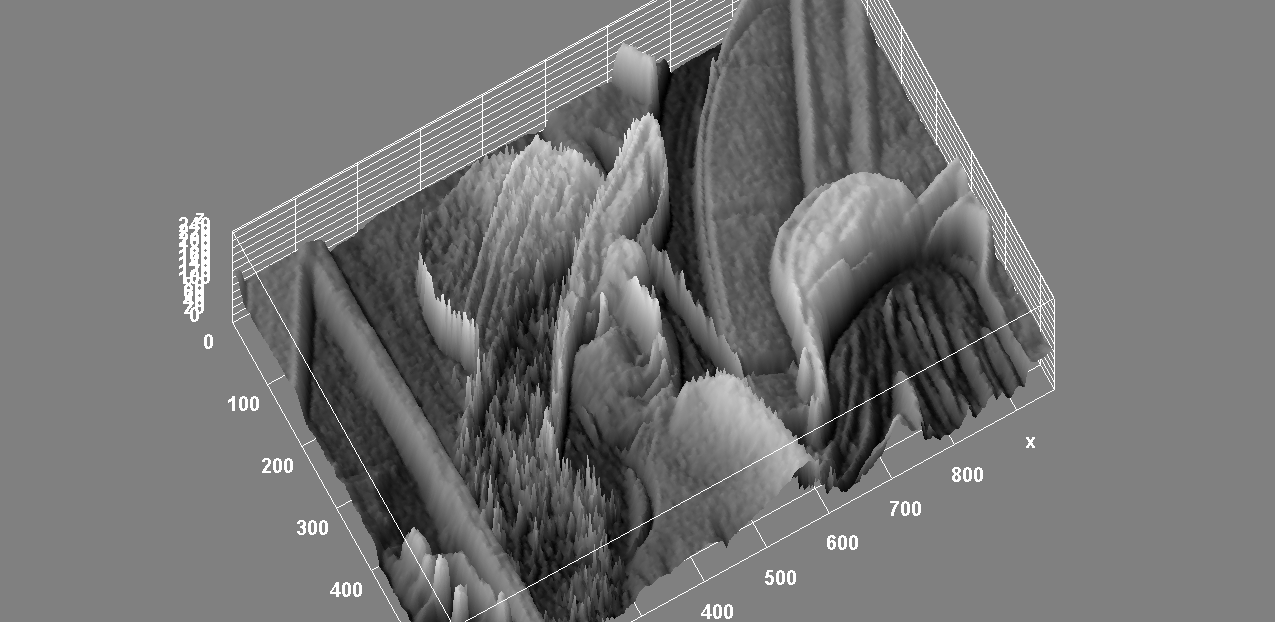
\includegraphics[width=0.7\linewidth]{img/img1}
		\caption{Representação das dimensões da imagem e a intensidade de cada pixel}
		\label{fig:img1}
	\end{figure}
	
	Normalmente as imagens são utilizadas no sistema \textit{Red, Green and Blue} (RGB), isso significa que cada pixel é uma aproximação resultante das intensidades de vermelho, azul e verde. A união das três cores no pixel forma a imagem de 3 bandas \citep{biasi2002desenvolvimento}. Segundo \cite{de2006introduccao} a demonstração da imagem de três bandas pode ser a seguinte equação:
	\begin{equation}
	F(x,y)=F_r(x,y)+F_g(x,y)+F_b(x,y)
	\end{equation}
	
	
	A imagem \ref{fig:blue} demonstra as bandas de uma imagem colorida.
	

\begin{figure}[h!]
	\centering
	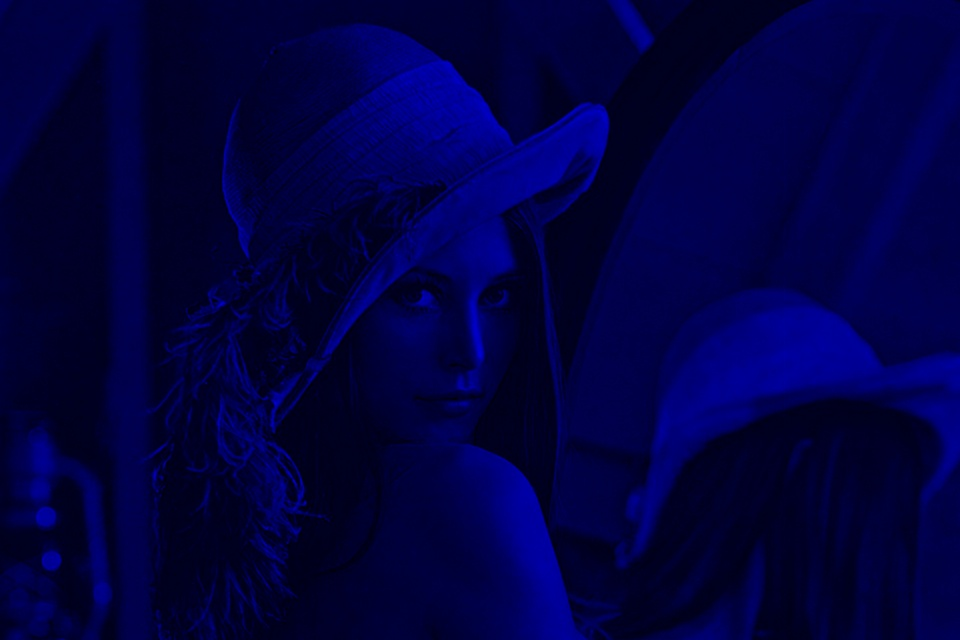
\includegraphics[width=0.4\linewidth]{img/Blue}
	\caption{Representação da banda azul}
	\label{fig:blue}
\end{figure}
\begin{figure}[h!]
	\centering
	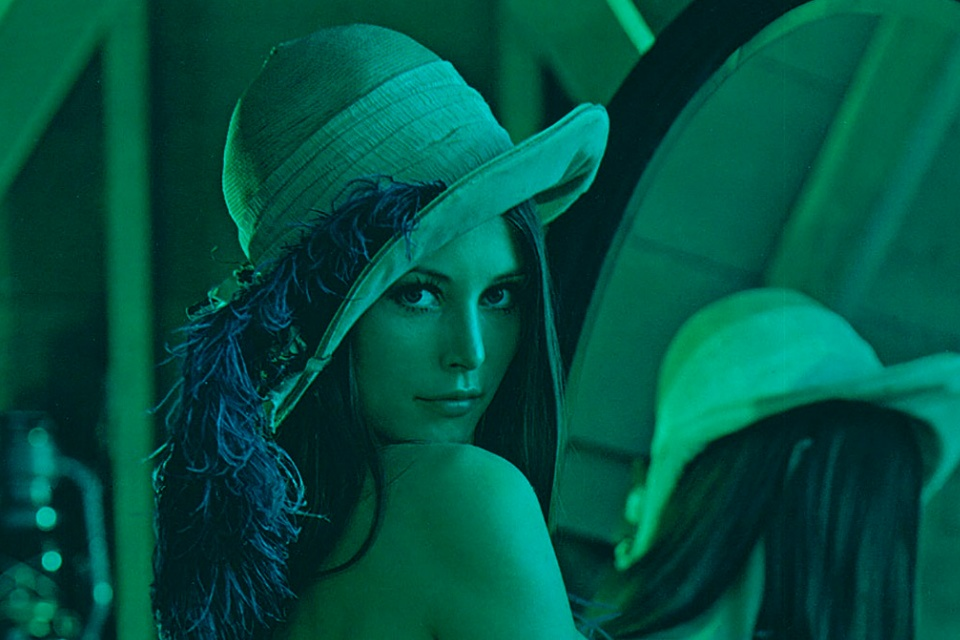
\includegraphics[width=0.4\linewidth]{img/gree}
	\caption{Representação da banda verde}
	\label{fig:gree}
\end{figure}
\begin{figure}[h!]
	\centering
	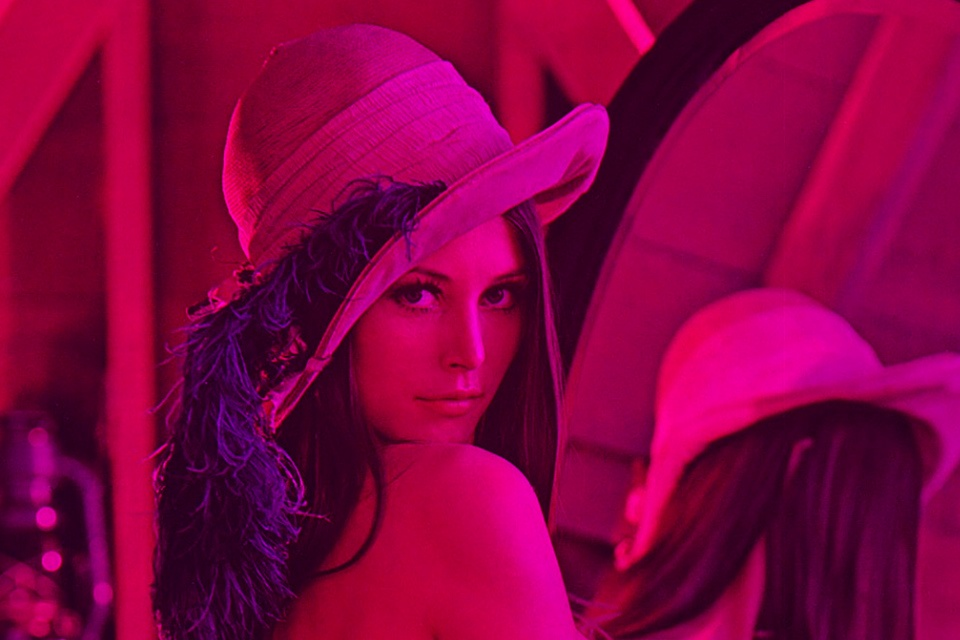
\includegraphics[width=0.4\linewidth]{img/Red}
	\caption{Representação da banda vermelha}
	\label{fig:red}
\end{figure}
	
	Majoritariamente as imagens utilizadas no trabalho foram de 8 bits, ou seja, elas suportam tonalidades de cores nas escalas RGB que variam de 0 a 255, totalizando $2^8$ tipos de cores. Segundo \cite{morgan2008tecnicas} O tamanho de um arquivo digital está diretamente relacionado com a qualidade dos detalhes visíveis e o tamanho do intervalo de cores, entretanto é importante ressaltar que o processamento de arquivos grandes demanda maior tempo, podendo ser inviável sua aplicação. Por convenção na área de computação visual adotou-se que a intensidade do pixel igual a 0 representaria o preto e o 255 representaria o branco, todas as outras cores são variações nesse intervalo. 
	
	Segundo \cite{de2006introduccao} existem duas classificações mais relevantes quando se trata de operações que manipulam de forma direta o pixel: as operações pontuais e as operações locais ou por máscaras. O objetivo desses cálculos é, por meio de uma sequência de funções aplicadas sobre os \textit{pixels} da fotografia original, criar uma imagem de saída que terá alguns parâmetros modificados. Nas operações pontuais cada elemento da imagem da saída estará em função apenas de um único elemento correspondente na imagem de entrada. Entretanto, nas operações locais o valor de saída é dependente não apenas do elemento correspondente na imagem de origem, mas também a vizinhança desse \textit{pixel}, isto é, os elementos que estão dentro da máscara. As máscaras são matrizes com dimensões pequenas que podem ser aplicadas em cada pixel da imagem \cite{silva2000segmentaccao}. A imagem a seguir exemplifica essa operação:
	
	\begin{figure}[h!]
		\centering
		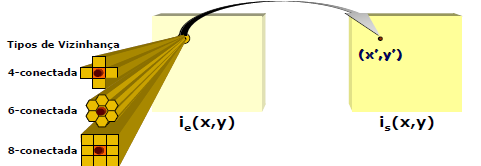
\includegraphics[width=0.7\linewidth]{img/f8d}
		\caption{Exemplo dos diagramas de transformação \citep{de2006introduccao}}
		\label{fig:f8d}
	\end{figure}
	
	Na aplicação da máscara o pixel a ser tratado é posicionado no centro da matriz de operação e o resultado se torna um novo pixel na mesma posição. 
	
	A par desses conceitos, o processamento se inicia transformando a imagem formada pelas bandas RGB em tons de cinza. Isso porque as variações entre as bandas serão analisadas apenas como uma variação de cinza. Segundo o site oficial do Matlab \cite{Matlab} a transformação que a biblioteca incluída no algoritmo aplica é baseada em uma média ponderada das componentes RGB de cada pixel, dada pela fórmula a seguir:
	
	\begin{equation}
	F(x,y)=(0,299*F_r(x,y))+(0,057*F_g(x,y))+(0,114*F_b(x,y))
	\end{equation} 
			
	Após a transformação em escalas de cinza inicia-se a aplicação dos métodos para a detecção de borda, o grupo escolheu o método criado por John Canny uma vez que os parâmetros ótimos desse processo supriam as necessidades do nosso objetivo.  Esses parâmetros serão detalhados nos tópicos seguintes. A imagem que o Método resulta na saída é denominada imagem binária, isso porque os elementos variam entre 0 e 1, de forma que o 1 representa que naquele espaço há uma borda.
	
	\begin{figure}[h!]
		\centering
		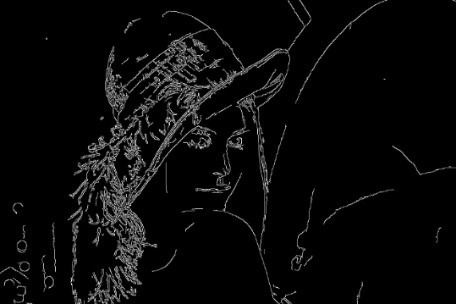
\includegraphics[width=0.7\linewidth]{img/img9}
		\caption{Imagem resultante do Método Canny}
		\label{fig:img9}
	\end{figure}
	
	
	\subsection{Método Canny para a detecção de borda}
	Canny apresentou a primeira ideia sobre detecção de borda em 1983 em seu artigo denominado \textit{A variational approach to edge detection} \citep{canny1983variational}. Nesse artigo são apresentados três parâmetros que Canny considera como sendo um filtro ideal para a detecção de borda. (1) O filtro deveria ter a menor taxa de erro possível, de forma a retornar a maior quantidade de bordas verdadeiras de uma imagem, considerando verdade uma borda proveniente da variação de cor entre um objeto e um segundo plano. Além disso, (2) a posição dos pixels marcados com variações de cores deve estar ao centro da borda. Por fim, (3) a borda deveria ter como espessura o tamanho de um pixel. 
	
	Para o retorno de uma imagem binária, representando as bordas de objetos, o método Canny realiza quatro tipos de operações sobre a fotografia original. Veja nos tópicos a seguir.  
	
	\subsubsection{Suavização Gaussiana}
	A primeira operação aplicada sobre a imagem é a filtragem conhecida como uma Suavização Gaussiana, que terá como objetivo diminuir ruídos sobre a imagem e facilitar a detecção de bordas. Por ruídos, entende-se como sendo frequências muito altas de variações de cores. A suavização se baseia em tirar a média ponderada da intensidade de cada pixel com os seus vizinhos. Diferente da transformação em escala de cinza que tirava a média ponderada da escala RGB do \textit{pixel}.  
	
	\subsubsection{Convolução}
	Na próxima etapa, aplica-se a ideia de convolução sobre a imagem, de forma que uma matriz de operação 3x3 filtra \textit{pixel} a \textit{pixel} e encontra uma relação entre o elemento e a intensidade de variação dos seus oito vizinhos \cite{do2002processo}, levando em consideração pesos para cada um desses, o que equivale a primeira derivada.
	
	\begin{figure}[h!]
		\centering
		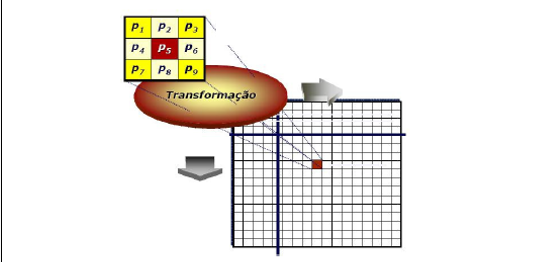
\includegraphics[width=0.7\linewidth]{img/img91}
		\caption{Exemplo da aplicação da convolução sobre uma imagem \citep{morgan2008tecnicas}}
		\label{fig:img91}
	\end{figure}
	
	As imagens são formadas por duas dimensões, dessa forma para melhorar o processo de encontrar a variação da intensidade de cor se aplicar a convolução nos dois eixos, x e y, simulando uma derivada parcial sobre a imagem \cite{biasi2002desenvolvimento}. O representante dessas derivadas será denominado gradiente, calculado como sendo o vetor resultante das derivadas em um certo \textit{pixel}. O gradiente pode ser dado por:
	
	\begin{equation}
	\bigtriangledown A(x,y)=\frac{dA}{dx},\frac{dA}{dy}
	\end{equation}
	
	Essa fórmula apresenta o gradiente no \textit{pixel} A(x,y) com componente x igual à derivada do pixel em função do eixo x e y igual a derivada do mesmo pixel em função de y. O tamanho do gradiente identifica a intensidade da derivada sobre um elemento na imagem, além disso, o seu sentido e direção aponta para onde há a maior variação de cor \cite{de2006introduccao}.
	
	\begin{equation}
	\mid G \mid= \sqrt{Gx^2+Gy^2}
	\end{equation}
	
	\begin{equation}
	 \theta = \arctan \frac{Gy}{Gx}
	\end{equation}
	
	É importante ressaltar que como tratamos cada pixel da imagem como um elemento de uma matriz, o ângulo do gradiente é limitado em 0, 45, 90 e 135, considerando apenas o primeiro e segundo quadrante. Dessa forma, quando $\theta$ resulta em um ângulo diferente desses há um arredondamento, isso pode ser visto na imagem \ref{fig:im10}.
	
	\begin{figure}[h!]
		\centering
		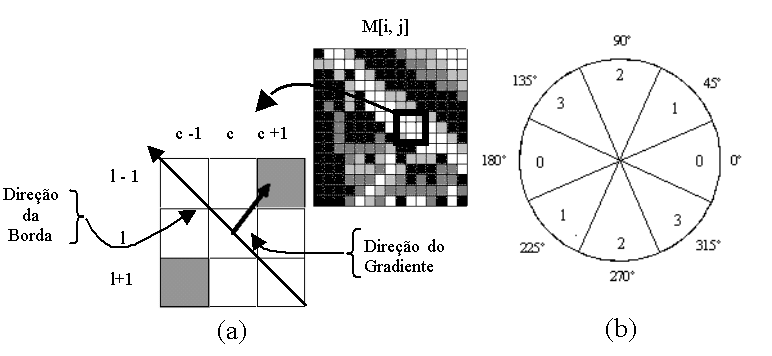
\includegraphics[width=0.7\linewidth]{img/im10}
		\caption{Direção do gradiente \citep{do2002processo}}
		\label{fig:im10}
	\end{figure}
	
	Existem diversos tipos de operadores para a detecção de gradiente, o que o grupo utiliza é o operador de Sobel que confere maior pesos aos vizinhos não nulos mais próximos, produzindo assim bordas diagonais menos intensas \cite{de2006introduccao}.
	
\begin{figure}[h!]
	\centering
	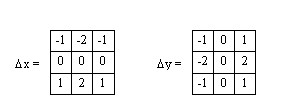
\includegraphics[width=0.7\linewidth]{img/FormatFactorysobel}
	\caption{Operador de convolução Sobel \citep{de2006introduccao}}
	\label{fig:formatfactorysobel}
\end{figure}
		
	
	\subsubsection{Supressão do não máximo}
	
	Após aplicar a convolução em toda a imagem se inicia o processo de filtrar os pontos que serão bordas. Inicialmente é feito supressão do não máximo, que zera todos os valores não máximos na direção do gradiente. Relembrando que os gradientes máximos serão os pontos onde houve maior variação na intensidade da cor em uma imagem. Essa supressão possibilita que a borda seja representada apenas por um único \textit{pixel}.
	
	\subsubsection{Limiarização}
	
	Por fim, há a limiarização, que segundo \cite{silva2000segmentaccao} são parâmetros que delimitam a atuação de procedimentos sobre a imagem. No contexto do grupo a limiarização define um intervalo de valores que são considerados como bordas na imagem. 
	
	Entretanto, um dos principais problemas é definir os valores que serviram de parâmetros, uma vez que determinadas variáveis podem interferir na qualidade da borda, como por exemplo, iluminação, qualidade da imagem e a distância do objeto até a câmera. Isto significa que, quando um mesmo sistema é colocado em ambientes diferentes a limiarização tende a não fornecer resultados similares \citep{silva2000segmentaccao}. 
	
	Após definir o intervalo acontece o processo conhecido com binarização da imagem, definido por \cite{silva2000segmentaccao}. Nessa etapa que há a separação do plano de fundo e do objeto, de forma que todos os valores diferentes de zero depois do processamento são considerados como borda e recebem o valor \textit{true} (1), e o restante \textit{false} (0).
	
	Segundo segmentação \cite{morgan2008tecnicas} matematicamente a detecção de borda pode ser definida como 
	
	\begin{equation}
	G(x,y)=\begin{cases} 1 & f(x,y)>T \\ 
	
	0 & f(x,y)\le T \end{cases}
	\end{equation}
	
	Onde f(x,y) é o pixel na posição x e y da imagem original, T é o parâmetro e G(x,y) é o pixel da imagem binária.
	
	\subsection{Biblioteca para o processamento de imagem: OpenCV}
	O OpenCV (\textit{Open Source Computer Vision Library}) pode ser utilizada em interfaces C++, Phyton e Java e é disponível para uso em Windows, Linux, Mac OS, iOS e Android. Sendo projetada para eficiência computacional, seu foco é trabalhar com aplicações em tempo real.
	
	\begin{quote}
		A biblioteca OpenCV foi desenvolvida pela Intel e possui mais de 500 funções [4]. Foi idealizada com o objetivo de tornar a visão computacional acessível a usuários e programadores em áreas tais como a interação humano-computador em tempo real e a robótica. A biblioteca está disponível com o código fonte e os executáveis (binários) otimizados para os processadores Intel. Um programa OpenCV, ao ser executado, invoca automaticamente uma DLL (Dynamic Linked Library) que detecta o tipo de processador e carrega, por sua vez, a DLL otimizada para este. Juntamente com o pacote OpenCV é oferecida a biblioteca IPL (Image Processing Library), da qual a OpenCV depende parcialmente, além de documentação e um conjunto de códigos exemplos. \citep{marengoni2009tutorial}
	\end{quote}
	
	Existem cinco grupos de funções para essa biblioteca, sendo eles: Processamento de imagens; Análise estrutural; Análise de movimento e rastreamento de objetos; Reconhecimento de padrões e Calibração de câmera e reconstrução 3D \citep{marengoni2009tutorial}.
	
	Como a OpenCV trabalha com a visão computacional, têm-se diversas maneiras de se trabalhar com imagens. Em alguns casos analisa-se um quadro fixo carregado de algum lugar. Em outros trabalha-se com \textit{streaming} (modo ininterrupto de captar imagens de uma câmera) com dados em tempo real de algum dispositivo ou câmera. Na biblioteca mais especificamente, na parte HighGUI, é fornecida uma solução para essa situação \citep{bradski2008learning}. 
	
	O HighGUI pode ser dividido em três partes: hardware, sistema de arquivo e GUI. A parte do hardware está relacionada com o funcionamento das câmeras. O HighGUI permite uma maneira fácil de consultar recuperar a imagem mais recente da câmera. A parte do sistema de arquivo carrega e salva imagens.  Uma característica da biblioteca é que se podem ler vídeos usando os mesmos métodos que se utiliza para ler uma câmera. Portanto se abstrai do dispositivo utilizado e continua-se escrevendo um código interessante. A parte GUI é o sistema de janelas que fornece funções que permitem abrir uma janela e abrir uma imagem dentro dessa janela. Com isso é permitido responder a comandos com o mouse e teclado \citep{bradski2008learning}.
	
	
	\section{Metodologia}
	Como apresentado, o objetivo geral deste trabalho é demonstrar a aplicação do cálculo de derivadas na área da Engenharia de Computação, de forma a apresentar uma aplicação prática da diferenciação. Com esse intuito, foi realizada uma pesquisa experimental para aplicar o conhecimento adquirido através da literatura baseada em processamento de imagens. Além disso, um dos objetivos específicos foi desenvolver um algoritmo capaz de encontrar as bordas de um objeto em uma imagem e com isso retornar a medição de sua altura, demonstrando de forma simplista uma aplicação dos dados extraídos de uma imagem processada.
	
	A detecção da variação de intensidade em imagens é algo canônico na visão computacional \citep{canny1986computational}, e é baseado nos estudos do método aplicado por John Canny para detecção de bordas que foram realizadas as experimentações. Retomando o objetivo geral do trabalho, o entendimento do método Canny foi necessário, dado que este se baseia na aplicação da primeira derivada da função Gaussiana.
	
	Inicialmente os primeiros algoritmos foram desenvolvidos no software Scilab, pois além de gratuito, possui uma maneira simples para demonstrações matriciais e gráficas. Este software integra cálculo com matrizes, construção de gráficos e análises numéricas em um ambiente de fácil manipulação. A sua utilização foi essencial para o desenvolvimento do trabalho, pois simplificou a visualização da maneira que uma imagem é interpretada numericamente por um computador.
	
	A primeira etapa foi dedicada para implementação de um algoritmo que através da manipulação da matriz de uma imagem, retornasse uma matriz resultante apenas com elementos binários. Utilizando uma biblioteca própria para processamento de imagens no software Scilab, foi desenvolvido um algoritmo que recebe uma imagem e a salva na forma matricial, onde cada \textit{pixel} representa um elemento da matriz. O número atribuído a esse pixel, ou seja, ao elemento dessa matriz, é um valor do sistema RGB. Na sequência, utiliza-se um comando para transformar o valor RGB em um representante na escala de cinza, através da média ponderada entre as intensidades de vermelho, verde e azul. Essa modificação é necessária para diminuir as variações entre as cores dos \textit{pixels}. Por fim, é aplicado o método Canny, que é capaz de identificar mudanças na intensidade dos \textit{pixels} da imagem para detectar a presença de bordas.
	
	Após a demonstração das formas matriciais que uma imagem assume em um computador, seja em cores ou na escala de cinza, espera-se que os alunos sejam capazes de perceber uma das diversas aplicações possíveis do cálculo de derivada para encontrar as bordas presentes na imagem.
	
	\begin{figure}[h!]
		\centering
		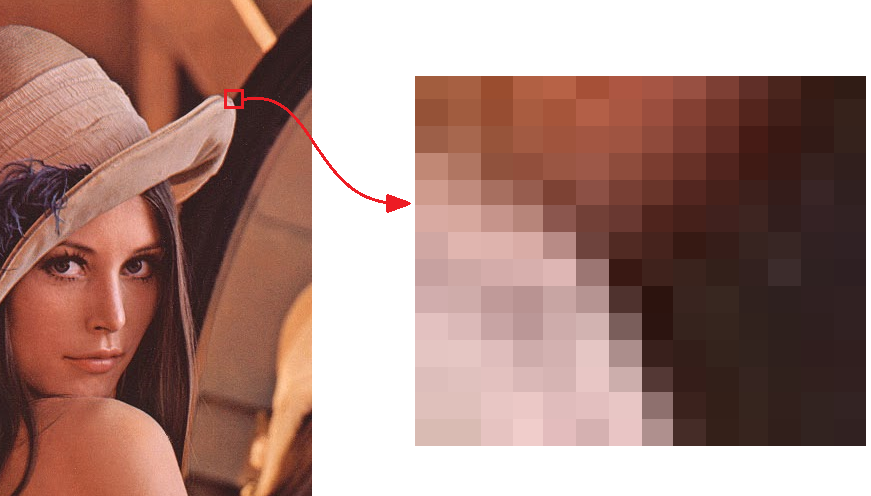
\includegraphics[width=0.5\linewidth]{img/F1}
		\caption{Detalhe de uma imagem para a visualização dos pixels}
		\label{fig:f1}
	\end{figure}
	 
	 \begin{figure}[h!]
	 	\centering
	 	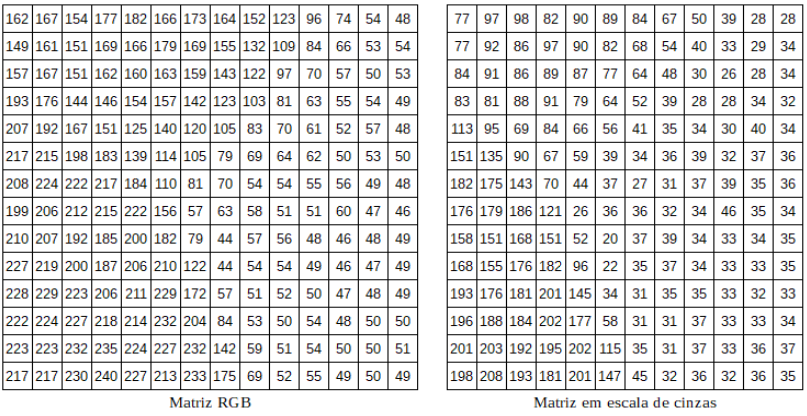
\includegraphics[width=0.9\linewidth]{img/F2}
	 	\caption{Matriz representante do recorte da figura \ref{fig:f1}}
	 	\label{fig:f2}
	 \end{figure}
	 
	\begin{figure}[h!]
		\centering
		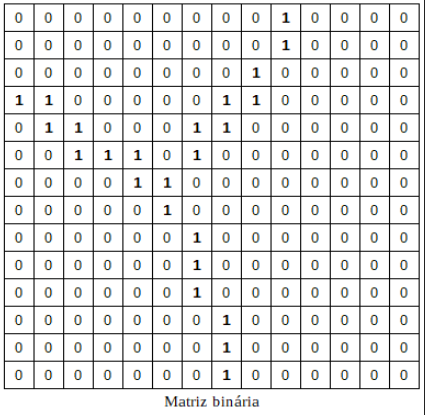
\includegraphics[width=0.4\linewidth]{img/F3}
		\caption{Matriz binaria do recorte da figura \ref{fig:f1}}
		\label{fig:f3}
	\end{figure}
	
	Ficou decidido durante a realização do projeto a substituição do software Scilab por um software capaz de copilar a linguagem de programação C++. Essa decisão foi tomada pelo fato de essa linguagem trabalhar com a biblioteca OpenCV. Como explicado, essa biblioteca possui eficiência para aplicações em tempo real e, além disso, a linguagem C++ demanda menos processamento e é orientada à objeto o que amplia as possibilidades a serem trabalhadas.
	
	\section{Resultados}
	
	Retomando um dos objetivos específicos deste trabalho, utilizamos a matriz binária gerada para realizar a medição de um objeto contido na imagem. A matriz resultante da aplicação do método Canny é uma matriz contendo apenas zeros e uns, onde zero representa a ausência de borda e um a presença. Sabendo disso, foi criada uma função que retornava a primeira e a última linha da matriz que contém o elemento um, ou seja, o elemento que indica a primeira e última borda do objeto. Com essas informações foi possível, através de subtração, encontrar a altura do objeto dada em \textit{pixels}.
	
	Foram realizadas diversas experimentações para constatar a correlação entre a altura em \textit{pixels}, e a altura real do objeto em milímetros. Para esse processo, foi necessário o controle de algumas variáveis, como: a distância do objeto à câmera; a rotação do objeto; e o processo de limiarização do método Canny.
	
	
	\begin{table}[h!]
		\begin{tabular}{lcccl}
			\cline{1-4}
			\multicolumn{1}{|l|}{Objeto}            & \multicolumn{1}{c|}{Tamanho (mm)} & \multicolumn{1}{c|}{Medida em pixels} & \multicolumn{1}{c|}{Relação Pixel/mm} &  \\ \cline{1-4}
			\multicolumn{1}{|l|}{A4 horizontal}     & \multicolumn{1}{c|}{210}          & \multicolumn{1}{c|}{280}              & \multicolumn{1}{c|}{0,75}             &  \\ \cline{1-4}
			\multicolumn{1}{|l|}{A4 vertical}       & \multicolumn{1}{c|}{294}          & \multicolumn{1}{c|}{394}              & \multicolumn{1}{c|}{0,75}             &  \\ \cline{1-4}
			\multicolumn{1}{|l|}{Celular}           & \multicolumn{1}{c|}{140}          & \multicolumn{1}{c|}{185}              & \multicolumn{1}{c|}{0,76}             &  \\ \cline{1-4}
			\multicolumn{1}{|l|}{Cartão vertical}   & \multicolumn{1}{c|}{94}           & \multicolumn{1}{c|}{124}              & \multicolumn{1}{c|}{0,76}             &  \\ \cline{1-4}
			\multicolumn{1}{|l|}{Cartão horizontal} & \multicolumn{1}{c|}{66}           & \multicolumn{1}{c|}{88}               & \multicolumn{1}{c|}{0,75}             &  \\ \cline{1-4}
			\multicolumn{1}{c}{}                    &                                   &                                       &                                       &  \\ \cline{3-4}
			\multicolumn{1}{c}{}                    & \multicolumn{1}{c|}{}             & \multicolumn{1}{c|}{Média:}           & \multicolumn{1}{c|}{0,75}             &  \\ \cline{3-4}
			\multicolumn{1}{c}{}                    & \multicolumn{1}{c|}{}             & \multicolumn{1}{c|}{Desv. Padrão:}    & \multicolumn{1}{c|}{0,005}            &  \\ \cline{3-4}
		\end{tabular}
		\caption{Resultado das medições realizadas à 500 milímetros de distância.}
		\label{t1}
	\end{table}
	
	
	
	\begin{table}[h!]
		\begin{tabular}{lcccl}
			\cline{1-4}
			\multicolumn{1}{|l|}{Objeto}            & \multicolumn{1}{c|}{Tamanho (mm)} & \multicolumn{1}{c|}{Medida em pixels} & \multicolumn{1}{c|}{Relação Pixel/mm} &  \\ \cline{1-4}
			\multicolumn{1}{|l|}{A4 horizontal}     & \multicolumn{1}{c|}{210}          & \multicolumn{1}{c|}{191}              & \multicolumn{1}{c|}{1,10}             &  \\ \cline{1-4}
			\multicolumn{1}{|l|}{A4 vertical}       & \multicolumn{1}{c|}{294}          & \multicolumn{1}{c|}{269}              & \multicolumn{1}{c|}{1,09}             &  \\ \cline{1-4}
			\multicolumn{1}{|l|}{Celular}           & \multicolumn{1}{c|}{140}          & \multicolumn{1}{c|}{126}              & \multicolumn{1}{c|}{1,11}             &  \\ \cline{1-4}
			\multicolumn{1}{|l|}{Cartão vertical}   & \multicolumn{1}{c|}{94}           & \multicolumn{1}{c|}{86}               & \multicolumn{1}{c|}{1,09}             &  \\ \cline{1-4}
			\multicolumn{1}{|l|}{Cartão horizontal} & \multicolumn{1}{c|}{66}           & \multicolumn{1}{c|}{61}               & \multicolumn{1}{c|}{1,08}             &  \\ \cline{1-4}
			\multicolumn{1}{c}{}                    &                                   &                                       &                                       &  \\ \cline{3-4}
			\multicolumn{1}{c}{}                    & \multicolumn{1}{c|}{}             & \multicolumn{1}{c|}{Média:}           & \multicolumn{1}{c|}{1,10}             &  \\ \cline{3-4}
			\multicolumn{1}{c}{}                    & \multicolumn{1}{c|}{}             & \multicolumn{1}{c|}{Desv. Padrão:}    & \multicolumn{1}{c|}{0,011}            &  \\ \cline{3-4}
		\end{tabular}
		\caption{Resultado das medições realizadas à 700 milímetros de distância.}
		\label{t2}
	\end{table}
	
	
	\begin{table}[h!]
		\begin{tabular}{lcccl}
			\cline{1-4}
			\multicolumn{1}{|l|}{Objeto}            & \multicolumn{1}{c|}{Tamanho (mm)} & \multicolumn{1}{c|}{Medida em pixels} & \multicolumn{1}{c|}{Relação Pixel/mm} &  \\ \cline{1-4}
			\multicolumn{1}{|l|}{A4 horizontal}     & \multicolumn{1}{c|}{210}          & \multicolumn{1}{c|}{142}              & \multicolumn{1}{c|}{1,48}             &  \\ \cline{1-4}
			\multicolumn{1}{|l|}{A4 vertical}       & \multicolumn{1}{c|}{294}          & \multicolumn{1}{c|}{188}              & \multicolumn{1}{c|}{1,56}             &  \\ \cline{1-4}
			\multicolumn{1}{|l|}{Celular}           & \multicolumn{1}{c|}{140}          & \multicolumn{1}{c|}{91}               & \multicolumn{1}{c|}{1,54}             &  \\ \cline{1-4}
			\multicolumn{1}{|l|}{Cartão vertical}   & \multicolumn{1}{c|}{94}           & \multicolumn{1}{c|}{64}               & \multicolumn{1}{c|}{1,47}             &  \\ \cline{1-4}
			\multicolumn{1}{|l|}{Cartão horizontal} & \multicolumn{1}{c|}{66}           & \multicolumn{1}{c|}{45}               & \multicolumn{1}{c|}{1,47}             &  \\ \cline{1-4}
			\multicolumn{1}{c}{}                    &                                   &                                       &                                       &  \\ \cline{3-4}
			\multicolumn{1}{c}{}                    & \multicolumn{1}{c|}{}             & \multicolumn{1}{c|}{Média:}           & \multicolumn{1}{c|}{1,49}             &  \\ \cline{3-4}
			\multicolumn{1}{c}{}                    & \multicolumn{1}{c|}{}             & \multicolumn{1}{c|}{Desv. Padrão:}    & \multicolumn{1}{c|}{0,045}            &  \\ \cline{3-4}
		\end{tabular}
		\caption{Resultado das medições realizadas à 1000 milímetros de distância.}
		\label{t3}
	\end{table}
	
	
	Como pode ser observado na Tabela 1, o desvio padrão da relação pixel/milímetros é bem inferior àquela constatada na Tabela 3. Isso indica que quanto mais próximo a câmera estiver do objeto medido, maior será a repetitividade do processo, assim como melhor será a precisão. Isso está relacionado com a perda de detalhes do objeto ao afastá-lo da câmera. Em posse dessas informações, foi decidido realizar a medição de objetos em tempo real, e não mais utilizar imagens estáticas. Para esse processo, foi necessário criar uma etapa para estabelecer uma relação inicial entre \textit{pixels} e centímetros para ser mantida durante a medição de novos objetos. Este processo consiste na utilização de um objeto com dimensões conhecidas, e a partir da medição deste objeto dada em \textit{pixels} computar a relação entre pixel e centímetro a ser mantida.
	
	\begin{figure}[hh!]
		\centering
		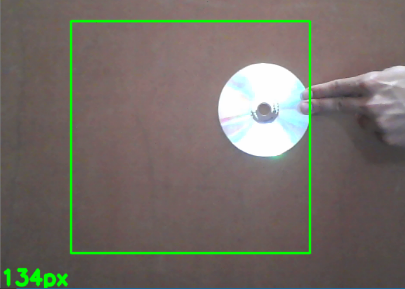
\includegraphics[width=0.7\linewidth]{img/F4}
		\caption{ Computando altura em pixels para ser utilizado como referência}
		\label{fig:f4}
	\end{figure}

	
	\begin{figure}[hh!]
		\centering
		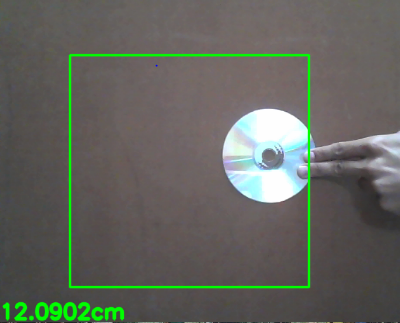
\includegraphics[width=0.7\linewidth]{img/F5}
		\caption{Criando relação cm/px}
		\label{fig:f5}
	\end{figure}
	
	\begin{figure}[hh!]
		\centering
		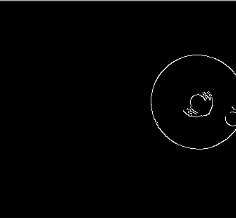
\includegraphics[width=0.4\linewidth]{img/F6}
		\caption{Bordas extraídas de um objeto}
		\label{fig:f6}
	\end{figure}
	

	Na figura \ref{fig:f4}, o diâmetro do CD foi equivalente à 134 pixels. Como um CD tem diâmetro de 12,0 centímetros, o software computou a relação pixel/centímetro equivalente à aproximadamente 0,089 cm/px. Isto significa que cada pixel equivale a 0,089 centímetro. Esta referenciação foi realizada com a câmera a uma distância de 750 milímetros do objeto, e mantida para as demais medições.
	
	Como as bordas que não representam o objeto, e as bordas do objeto são armazenadas da mesma maneira, para realizar as medições era necessário criar um ambiente em que as únicas bordas presentes fossem às do objeto desejado. Essa situação era devido ao fato de o algoritmo procurar o primeiro e o último elemento da matriz que representasse borda, e quando encontrado falsas bordas, ou bordas que não representam o objeto, falhas são geradas. Percebido isso, foi desenvolvido uma nova função no programa que é responsável por delimitar a área de interesse. Esta função tem como simples objetivo reduzir a área de busca por bordas, transformando a matriz da imagem em uma matriz menor em que objeto se encontra inserido.
	
	\begin{figure}[h!]
		\centering
		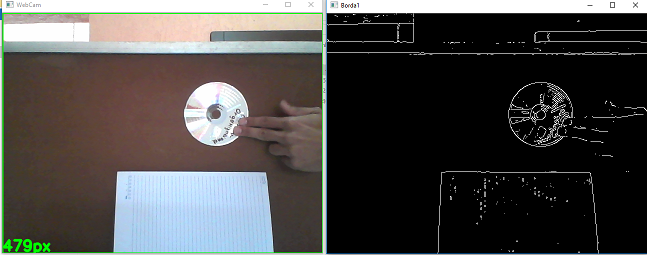
\includegraphics[width=0.7\linewidth]{img/F7}
		\caption{Detecção de bordas sem delimitação de área}
		\label{fig:f7}
	\end{figure}
	
	\begin{figure}[h!]
		\centering
		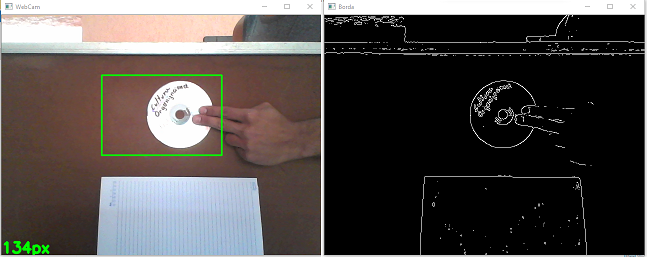
\includegraphics[width=0.7\linewidth]{img/F8}
		\caption{Delimitação da área de busca por bordas do objeto}
		\label{fig:f8}
	\end{figure}
	
	\begin{figure}[h!]
		\centering
		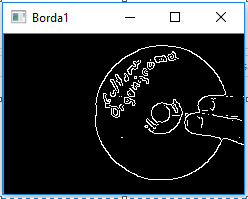
\includegraphics[width=0.25\linewidth]{img/F9}
		\caption{Imagem representante da área delimitada na figura \ref{fig:f8}}
		\label{fig:f9}
	\end{figure}
		
	Como pode ser observado na figura \ref{fig:f7}, onde não há delimitação da área de busca, o algoritmo retorna uma altura em pixels equivalente à 479px. Já na figura \ref{fig:f8}, a região de busca por bordas corresponde à área interna do retângulo de contorno verde, isso significa que somente o que estiver compreendido na figura \ref{fig:f9} será analisado.
	
	Além do problema com a área de interesse, houve também a necessidade de permitir que o usuário pudesse parametrizar, quando necessário, a limiarização desejada para o processo. Pois, a aplicação da limiarização é difícil e envolve experimentação. “A permanência de falsas bordas, após a limiarização, pode ter como motivo a escolha de um limiar baixo, ou alto demais” \citep[p. 9]{do2002processo}. Na figura \ref{fig:f10} é possível perceber o impacto de uma limiarização mal aplicada. Na imagem à esquerda as bordas ficam restritas ao objeto, já na imagem à direita, ocorre a presença de falsas bordas, o que interfere na medição.
	
	\begin{figure}[h!]
		\centering
		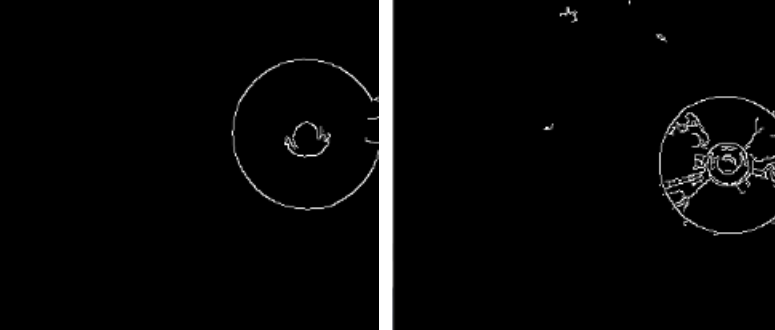
\includegraphics[width=0.7\linewidth]{img/F10}
		\caption{Diferenças de limiarização e presença de falsas bordas}
		\label{fig:f10}
	\end{figure}
			
	Por fim, reduzindo a área de busca, e ajustando a limiarização durante o processo de medição, o algoritmo foi capaz de retornar medições dos objetos com uma precisão de  0,0975 centímetro, ou seja, inferior à 1 milímetro (vide Tabela 4), o que consiste em um resultado aceitável, visto que era buscado a demonstração de um processo possível. Porém, o fato de trabalharmos com uma câmera 2D, implica na perda de percepção de profundidade. Logo, quando há rotação do objeto a medição passa a se invalidar. Aprofundar os cálculos para encontrar medições do objeto mesmo com rotações, é uma das possíveis vertentes que este trabalho poderá seguir, portanto não será abordado essa variável de processo. 
	
	\begin{table}[]
		\begin{tabular}{lcccl}
			\cline{1-4}
			\multicolumn{1}{|l|}{Objeto}                      & \multicolumn{1}{c|}{Esperado (cm)} & \multicolumn{1}{c|}{Medido (cm)} & \multicolumn{1}{c|}{Erro (cm)} &  \\ \cline{1-4}
			\multicolumn{1}{|l|}{CD Padrão}                   & \multicolumn{1}{c|}{12,00}         & \multicolumn{1}{c|}{12,09}       & \multicolumn{1}{c|}{0,09}      &  \\ \cline{1-4}
			\multicolumn{1}{|l|}{Mini CD}                     & \multicolumn{1}{c|}{8,00}          & \multicolumn{1}{c|}{8,03}        & \multicolumn{1}{c|}{0,03}      &  \\ \cline{1-4}
			\multicolumn{1}{|l|}{CC Horizontal}               & \multicolumn{1}{c|}{5,40}          & \multicolumn{1}{c|}{5,50}        & \multicolumn{1}{c|}{0,10}      &  \\ \cline{1-4}
			\multicolumn{1}{|l|}{CC Vertical}                 & \multicolumn{1}{c|}{8,56}          & \multicolumn{1}{c|}{8,66}        & \multicolumn{1}{c|}{0,10}      &  \\ \cline{1-4}
			\multicolumn{1}{|l|}{A4 Horizontal}               & \multicolumn{1}{c|}{21,00}         & \multicolumn{1}{c|}{21,11}       & \multicolumn{1}{c|}{0,11}      &  \\ \cline{1-4}
			\multicolumn{1}{|l|}{A4 Vertical}                 & \multicolumn{1}{c|}{29,70}         & \multicolumn{1}{c|}{29,77}       & \multicolumn{1}{c|}{0,07}      &  \\ \cline{1-4}
			\multicolumn{1}{|l|}{Cartão de visita Horizontal} & \multicolumn{1}{c|}{4,80}          & \multicolumn{1}{c|}{4,96}        & \multicolumn{1}{c|}{0,16}      &  \\ \cline{1-4}
			\multicolumn{1}{|l|}{Cartão de visita Vertical}   & \multicolumn{1}{c|}{8,90}          & \multicolumn{1}{c|}{9,02}        & \multicolumn{1}{c|}{0,12}      &  \\ \cline{1-4}
			\multicolumn{1}{c}{}                              &                                    &                                  &                                &  \\ \cline{3-4}
			\multicolumn{1}{c}{}                              & \multicolumn{1}{c|}{}              & \multicolumn{1}{c|}{Média}       & \multicolumn{1}{c|}{0,0975}    &  \\ \cline{3-4}
		\end{tabular}
		\caption{Resultados das medições realizadas}
		\label{t4}
	\end{table}
		
	\section{Considerações Finais}
	
	As imagens transmitem diversas informações sobre o mundo, como fatores históricos e culturais de uma determinada sociedade, noções biológicas de um ser vivo utilizando o raio – x, ou ainda informações da estrutura física de determinados objetos. O intuito desse trabalho era entender como a derivada poderia auxiliar no estudo dessa última informação, esclarecendo para os alunos do primeiro ano a aplicabilidade do Cálculo na Engenharia de Computação.
	
	A área de foco foi o processamento de imagem, mas especificamente a detecção de bordas utilizando o método de Canny. Essa área possuía vantagens que possibilitava visualizar a derivada e exigia pouco conhecimento para entender, de forma básica, como se produzia uma imagem de bordas como saída do processamento. Além disso, outra razão pela escolha dessa área, foi a possibilidade de visualizar o processamento de imagens capturadas pela Webcam, o que possibilitariam aos alunos avaliar, por meio de algoritmos, o ambiente ao seu redor em tempo real. A análise proposta por esse trabalho foi utilizar o método Canny para medir objetos. 
	
	A principal dificuldade encontrada foi conseguir filtrar as informações necessárias para se ter uma base do processamento sem que fosse exigido muito conhecimento. Além disso, o grupo entrou em contato com dificuldades existentes na área de computação visual, como: ruídos na imagem, bordas não desejadas, relação entre o tamanho do objeto e sua distância da câmera e etc.
	
	Portanto, por meio desse trabalho foi possível constatar que o processamento de imagem é uma área promissora que integra os conceitos do Cálculo da derivada e a área da computação. Como estudos futuros, o grupo pretende aperfeiçoar as técnicas de processamento utilizadas nesse trabalho, embarcando conceitos de outros períodos, além do primeiro e segundo. As melhorias que o grupo almeja são (1) conseguir fazer medições podendo varia a rotação do corpo e a distância desse até a câmera sem a necessidade de configurar uma nova relação; (2) automatizar a limiarização de bordas para cada ambiente; por fim (3) otimizar as estruturas do algoritmo.
	
	\bibliographystyle{sbc}
	\bibliography{sbc-template}
	
\end{document}
